\documentclass{standalone}
\usepackage{tikz}
\usetikzlibrary{shapes.geometric}

\newcommand{\bt}{\mathbf{t}}
\newcommand{\bx}{\mathbf{x}}
\newcommand{\by}{\mathbf{y}}
\newcommand{\bz}{\mathbf{z}}
\newcommand{\eq}{=}


\begin{document}
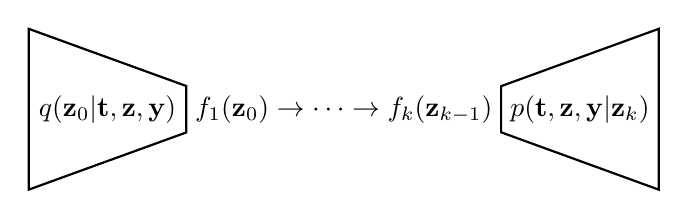
\begin{tikzpicture}
      \node [trapezium, trapezium left angle=-70, trapezium right angle=-70, minimum width=2cm, minimum height=2cm, draw, thick, rotate=90] (q) at (0, 0) {\rotatebox{-90}{$q(\bz_0|\bt, \bz, \by)$}};
      \node [trapezium, trapezium left angle=70, trapezium right angle=70, minimum width=2cm, minimum height=2cm, draw, thick, rotate=90] (p) at (6, 0) {\rotatebox{-90}{$p(\bt, \bz, \by| \bz_k)$}};
      \node[] (z) at (3, 0) {$f_1(\bz_0) \rightarrow  \cdots \rightarrow f_k(\bz_{k-1})$};
\end{tikzpicture}
\end{document}